
\section{Recovering Einsteinian Special Relativity}
Pursuant to the principle of maximal spatiotemporal symmetry, from this section onward we specialize to a $p=3, q=3$ dimensional spacetime, recovering Einsteinian special relativity through the compatibility of spacetime norms.

\subsection{Classical Causal Time}
In the rest frame $\mathrm{O}$, the temporal displacement takes the form
\begin{equation}\label{eq_temporal_displacement_vector}
    \mathbf{x}_{t} \coloneqq x^{n}\mathbf{e}_{n}, \quad x^{n} = ct^{n}, \quad n \in \{4,5,6\},
\end{equation}
anchored by fixed, mutually orthogonal temporal basis vectors satisfying $\mathbf{e}_{n}^{2} = +1$.

Selecting a fiducial unit vector $\mathbf{e}_{0}$ to mark the temporal orientation at a reference event $\tau_{0}$, we introduce the rotor
\begin{equation}
    \boldsymbol{\omega}_{t} = \exp(-\mathbf{i}(\tau)\theta^{t}(\tau)), \quad \mathbf{i}^{\dagger} = -\mathbf{i}, \quad \mathbf{i}^{2} = -1,
\end{equation}
where $\mathbf{i}$ denotes a smooth unit temporal bivector and $\theta^{t}$ signifies a real angle parametrized such that $\theta^{t}(\tau_{0}) = 0$, yielding $\boldsymbol{\omega}_{t}(\tau_{0}) = 1$. Its transformation determines the evolved unit vector
\begin{equation}\label{eq_pole_from_flag}
    \mathbf{e}_{t} = \boldsymbol{\omega}_{t}\mathbf{e}_{0}\boldsymbol{\omega}_{t}^{\dagger},
\end{equation}
which establishes the radial displacement
\begin{equation}
    \mathbf{x}_{t} = c r^{t}\mathbf{e}_{t}, \quad r^{t} = \sqrt{(t^{4})^{2} + (t^{5})^{2} + (t^{6})^{2}}.
\end{equation}
Comparing this relation against the expression $\mathbf{x}_{t} = x^{t}\mathbf{e}_{t} = ct\mathbf{e}_{t}$, previously employed for temporal translations, directly equates the magnitude $r^{t}$ with classical time $t$.

Upon introducing the unit volume element of the temporal subspace,
\begin{equation}
    \mathbf{I}_{t} = \mathbf{e}_{4}\mathbf{e}_{5}\mathbf{e}_{6},
\end{equation}
the rotational bivector can subsequently be formulated in terms of a real unit vector $\mathbf{n}_{t}(\tau)$ orthogonal to the plane of rotation generated by the rotor,
\begin{equation}
    \mathbf{i} = \mathbf{I}_{t}\mathbf{n}_{t}.
\end{equation}
Within a specified temporal basis, the causal vector possesses direction cosines
\begin{equation}
    \mathbf{e}_{0} = \hat{\vartheta}^{k}\mathbf{e}_{k}, \quad \hat{\vartheta}^{k} \coloneqq \frac{t^{k}}{t}, \quad \sum_{k=4}^{6}(\hat{\vartheta}^{k})^{2} = 1,
\end{equation}
corresponding to the generator
\begin{equation}
    \mathbf{i} = \mathbf{e}_{5}\mathbf{e}_{6}\hat{\vartheta}^{4} + \mathbf{e}_{6}\mathbf{e}_{4}\hat{\vartheta}^{5} + \mathbf{e}_{4}\mathbf{e}_{5}\hat{\vartheta}^{6}.
\end{equation}
At this juncture, $\mathbf{n}_{t}$ remains free to fluctuate along arbitrary direction cosines bounded only by $t = \sqrt{(t^{4})^{2} + (t^{5})^{2} + (t^{6})^{2}}$. Nevertheless, as demonstrated below, the invariant norm of the spacetime velocity fixes the causal temporal direction, leaving the residual rotation confined to a static plane possessing $\mathbf{e}_{0}$ as its normal.

\subsection{The Fixed Causal Time Direction}
Previously, we established that $\boldsymbol{\mathcal{U}}^{2}=\left(\mathrm{d}\boldsymbol{\mathcal{X}}/\mathrm{d}\tau\right)^{2}=c^{2}$. To determine the directional consequences of this invariant, we return to the linear six-position defined in Eq.~\eqref{eq_pq_position_def} and decompose the spatial displacement across its static basis,
\begin{equation}
    \boldsymbol{\mathcal{X}}=\mathbf{x}_{t}+\mathbf{x}_{s}=ct\mathbf{e}_{t}+x^{a}\mathbf{e}_{a},\quad a\in\{1,2,3\},
\end{equation}
which, using $\mathrm{d}t/\mathrm{d}\tau=\gamma$ alongside $\mathrm{d}x^{a}/\mathrm{d}t=u^{a}$ and denoting $\mathrm{d}/\mathrm{d}\tau$ by an overdot, gives
\begin{equation}\label{eq_six_velocity}
    \boldsymbol{\mathcal{U}}=\frac{\mathrm{d}\boldsymbol{\mathcal{X}}}{\mathrm{d}\tau}=\gamma(c\mathbf{e}_{t}+u^{a}\mathbf{e}_{a})+ct\dot{\mathbf{e}}_{t}.
\end{equation}
Since the temporal and spatial sectors are mutually orthogonal, with $\mathbf{e}_{t}^{2}=+1$ and $\mathbf{e}_{a}^{2}=-1$, while differentiation of the temporal unit norm gives $\mathbf{e}_{t}\cdot\dot{\mathbf{e}}_{t}=0$, squaring the six-velocity yields
\begin{equation}
    \boldsymbol{\mathcal{U}}^{2}=\gamma^{2}(c^{2}-u^{2})+c^{2}t^{2}\dot{\mathbf{e}}_{t}^{2}=c^{2},
\end{equation}
where the initial term already recovers the Lorentzian invariant $\gamma^{2}(c^{2}-u^{2})=c^{2}$.

Because the origin of $t$ is arbitrary and $\boldsymbol{\mathcal{U}}^{2}=c^{2}$ holds for all $t$, the remaining contribution vanishes identically, giving
\begin{equation}
    \dot{\mathbf{e}}_{t}^{2}=0,
\end{equation}
which, since $\dot{\mathbf{e}}_{t}$ lies within the positive-definite temporal subspace, implies
\begin{equation}\label{eq_compatibility_condition}
    \dot{\mathbf{e}}_{t}=0.
\end{equation}
Although this fixed orientation is expected in inertial frames, the comoving inertial frames corollary extends the result locally to accelerated observers, so the causal temporal direction remains fixed along the accelerated worldline.

\subsection{Four-Dimensional Spacetime}
\label{ch_causality_preservation}
Rather than immutably locking the temporal subspace, this compatibility requirement restricts relative temporal rotations strictly to the plane governed by $\mathbf{e}_{0}$ as its stationary normal. Consequently,
\begin{equation}\label{eq_pon_normal_fixed}
    \mathbf{n}_{t}\equiv\mathbf{e}_{0},\quad \mathbf{i}=\mathbf{I}_{t}\mathbf{e}_{0} \implies \hat{\vartheta}^{k} =\mathrm{constant}.
\end{equation}
Due to the constancy of these coefficients, each distinct temporal coordinate simplifies to
\begin{equation}
    t^{k}=\hat{\vartheta}^{k}t,
\end{equation}
and as a result, the three temporal coordinates collapse to a functional dependence on a single scalar $t$, even though the underlying temporal manifold remains inherently three-dimensional.

The emerging $(4+2)$-dimensional structure consists of a translational manifold spanned by $\mathbf{e}_{0}$ and $\mathbf{e}_{a}$, characterized by the four-position
\begin{equation}
    \mathbf{X}=\mathbf{e}_{\mu}X^{\mu}(\tau),\quad \mu\in\{0,1,2,3\},\quad X^{0}=ct(\tau),
\end{equation}
alongside a temporal plane orthogonal to $\mathbf{e}_{0}$, whose residual rotational motion is driven by $\mathbf{i}$ and parametrized by $\theta^{t}(\tau)$. This subspace, designated as the \emph{Plane-of-Now}, accommodates a continuous spectrum of frame orientations at a given causal time $t$, thereby extending the point-like notion of ``now'' in conventional Einsteinian kinematics.

Across the translational sector, the basis vectors obey the standard Minkowski Clifford algebra
\begin{equation}\label{eq_minkowski_metric}
    \mathbf{e}_{\mu}\mathbf{e}_{\nu}+\mathbf{e}_{\nu}\mathbf{e}_{\mu}=2\eta_{\mu\nu}^{\mathrm{4D}},\quad \eta_{\mu\nu}^{\mathrm{4D}}=\mathrm{diag}(+1,-1,-1,-1),
\end{equation}
and both, the four-position and its corresponding proper-time derivatives reproduce standard special-relativistic kinematics—with $\mathbf{e}_{0}$ fixing the primary light-cone orientation—while the Plane-of-Now furnishes the internal rotational dynamics foundational to the quantum-mechanical constructs addressed below.

Adopting a basis that sets $\mathbf{e}_{0} = \mathbf{e}_{4}$, the direction cosines simplify to
\begin{equation}
    \hat{\vartheta}^{4} = 1, \quad \hat{\vartheta}^{5} = 0, \quad \hat{\vartheta}^{6} = 0,
\end{equation}
with the Plane-of-Now spanned by $\{\mathbf{e}_{5}, \mathbf{e}_{6}\}$ and generated by $\mathbf{i} = \mathbf{e}_{5}\mathbf{e}_{6}$. Owing to its algebraic simplicity, this adapted frame will serve as the primary reference for explicit representations.

\subsection{Visualization of the Six-Dimensional Spacetime as a Flag-and-Pole System}
\label{ch_flag_pole_visualization}

\begin{figure}[htbp]
\centering

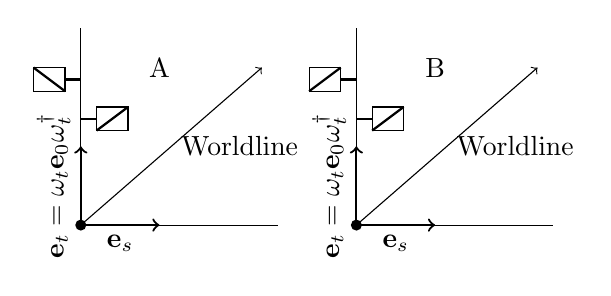
\begin{tikzpicture}
 % Define key coordinates A
 \coordinate (OriginA) at (0,0);
 \coordinate (TopYA) at (0,2.5);
 \coordinate (RighXA) at (2.5,0);
 \coordinate (StartWLA) at (0,0);
 \coordinate (EndWLA) at (2.3,2);

 % Flag 1 tips (Detached by 0.2, width 0.4)
 \coordinate (Flag1BottomLeft) at (0.2,1.2);
 \coordinate (Flag1BottomRight) at (0.6,1.2);
 \coordinate (Flag1TopLeft) at (0.2,1.5);
 \coordinate (Flag1TopRight) at (0.6,1.5);
 \coordinate (Arm1Pole) at (0,1.35);
 \coordinate (Arm1Flag) at (0.2,1.35);

 % Flag 2 tips
 \coordinate (Flag2BottomLeft) at (-0.2,1.7);
 \coordinate (Flag2BottomRight) at (-0.6,1.7);
 \coordinate (Flag2TopLeft) at (-0.2,2.0);
 \coordinate (Flag2TopRight) at (-0.6,2.0);
 \coordinate (Arm2Pole) at (0,1.85);
 \coordinate (Arm2Flag) at (-0.2,1.85);

 % Define key coordinates B
 \coordinate (OriginB) at (3.5,0);
 \coordinate (TopYB) at (3.5,2.5);
 \coordinate (RighXB) at (6.0,0);
 \coordinate (StartWLB) at (3.5,0);
 \coordinate (EndWLB) at (5.8,2);

 % Flag 3 tips
 \coordinate (Flag3BottomLeft) at (3.7,1.2);
 \coordinate (Flag3BottomRight) at (4.1,1.2);
 \coordinate (Flag3TopLeft) at (3.7,1.5);
 \coordinate (Flag3TopRight) at (4.1,1.5);
 \coordinate (Arm3Pole) at (3.5,1.35);
 \coordinate (Arm3Flag) at (3.7,1.35);

% Flag 4 tips
 \coordinate (Flag4BottomLeft) at (3.3,1.7);
 \coordinate (Flag4BottomRight) at (2.9,1.7);
 \coordinate (Flag4TopLeft) at (3.3,2.0);
 \coordinate (Flag4TopRight) at (2.9,2.0);
 \coordinate (Arm4Pole) at (3.5,1.85);
 \coordinate (Arm4Flag) at (3.3,1.85);
 
 % Draw the coordinate system A
 \fill (OriginA) circle (2pt) node[below left] {};
 \draw (OriginA) -- (RighXA);
 \draw (OriginA) -- (TopYA);
 \draw[thick, ->] (OriginA) -- ++(1,0) node[midway, below] {$\mathbf{e}_s$};
 \draw[thick, ->] (OriginA) -- ++(0,1) node[midway, left, rotate=90, anchor=south] {$\mathbf{e}_{t}=\boldsymbol{\omega}_{t}\mathbf{e}_{0}\boldsymbol{\omega}_{t}^{\dagger}$};
 
 % Draw Arm and Flag 1 (Scalar Base)
 \draw[thick] (Arm1Pole) -- (Arm1Flag);
 \draw (Flag1BottomRight) -- (Flag1BottomLeft) -- (Flag1TopLeft) -- (Flag1TopRight) -- cycle;
 \draw[thick] (Flag1BottomLeft) -- (Flag1TopRight);
 
 % Draw Arm and Flag 2 (Scalar Evolved - No Rotation)
 \draw[thick] (Arm2Pole) -- (Arm2Flag);
 \draw (Flag2BottomRight) -- (Flag2BottomLeft) -- (Flag2TopLeft) -- (Flag2TopRight) -- cycle;
 \draw[thick] (Flag2BottomLeft) -- (Flag2TopRight);
 
 % Draw worldline A
 \draw [->] (StartWLA) -- (EndWLA) node[midway, right] {Worldline};
 % Add an identification tag to diagram A
 \node at (1,2) {A};

 % Draw the coordinate system B
 \fill (OriginB) circle (2pt) node[below left] {};
 \draw (OriginB) -- (RighXB);
 \draw (OriginB) -- (TopYB);
 \draw[thick, ->] (OriginB) -- ++(1,0) node[midway, below] {$\mathbf{e}_s$};
 \draw[thick, ->] (OriginB) -- ++(0,1) node[midway, left, rotate=90, anchor=south] {$\mathbf{e}_{t}=\boldsymbol{\omega}_{t}\mathbf{e}_{0}\boldsymbol{\omega}_{t}^{\dagger}$};
 
 % Draw Arm and Flag 3 (Spinor Base)
 \draw[thick] (Arm3Pole) -- (Arm3Flag);
 \draw (Flag3BottomRight) -- (Flag3BottomLeft) -- (Flag3TopLeft) -- (Flag3TopRight) -- cycle;
 \draw[thick] (Flag3BottomLeft) -- (Flag3TopRight);
 
 % Draw Arm and Flag 4 (Spinor Twisted - 360 deg rotation)
 \draw[thick] (Arm4Pole) -- (Arm4Flag);
 \draw (Flag4BottomRight) -- (Flag4BottomLeft) -- (Flag4TopLeft) -- (Flag4TopRight) -- cycle;
 \draw[thick] (Flag4BottomRight) -- (Flag4TopLeft);


 % Draw worldline B
 \draw [->] (StartWLB) -- (EndWLB) node[midway, right] {Worldline};
 % Add an identification tag to diagram B
 \node at (4.5,2) {B};

\end{tikzpicture}

\caption{Flag-and-Pole depiction of the geometric framework. The stationary Pole direction $\mathbf{e}_{0}$ specifies the causal temporal axis and, in conjunction with the spatial frame (visualized as the ground), constitutes the Pole--ground coordinate system for the four-dimensional translational domain. The attached Flag embodies the temporal rotor $\boldsymbol{\omega}_{t}=\exp(-\mathbf{i}\theta^{t})$, whose operation produces the temporal vector $\mathbf{e}_{t}=\boldsymbol{\omega}_{t}\mathbf{e}_{0}\boldsymbol{\omega}_{t}^{\dagger}$. The angle $\theta^{t}$ parametrizes the angular movement of the Flag, whereas the generator $\mathbf{i}$ dictates its intrinsic algebraic rotation plane. Panels A and B depict alternative Flag configurations evaluated at identical proper time, highlighting how distinct rotational states map onto identical Pole--ground observables.}
\label{fig-FlagAndPoleDiag}
\end{figure}

With the causal temporal orientation locked via compatibility, Eq.~\eqref{eq_pole_from_flag} provides a vivid geometric representation of the temporal-frame architecture. In particular, the temporal space defined by $\mathbf{e}_{t}=\boldsymbol{\omega}_{t}\mathbf{e}_{0}\boldsymbol{\omega}_{t}^{\dagger}$, incorporating the rotor $\boldsymbol{\omega}_{t}=\exp(-\mathbf{i}\theta^{t})$, behaves precisely like a Flag-and-Pole system: the rigid Pole along $\mathbf{e}_{0}$ sets the causal temporal axis, whereas the attached Flag captures the action of the temporal rotor $\boldsymbol{\omega}_{t}$. Varying the orientation of the Flag through the parameter $\theta^{t}$ modulates the temporal rotational state without disturbing the underlying Pole--ground interval, while the generator $\mathbf{i}$—interpreted visually as an intrinsic twist within the Flag—governs the algebraic character of this rotation.

